
\documentclass[aspectratio=1610]{beamer}

\usepackage[english]{babel}
\usepackage[utf8]{inputenc}
\usepackage[T1]{fontenc}

\usepackage{lmodern}
\usepackage{amsmath,amsfonts,amssymb}

\usepackage{graphicx}
\usepackage{pgf}



%\usepackage[backend=biber, citestyle=authortitle-comp, bibstyle=authortitle]{biblatex}
%\usepackage{csquotes}
%\renewcommand{\bibliography}[1]{} % make noop. stillincl this cmd for
%\bibliography{../techdoc/bib/bibi}           % texnicenter to display the library
%\addbibresource{../techdoc/bib/bibi.bib}
%\bibhang1.5em 


%\usepackage[pdftex]{hyperref} %import last!
%\hypersetup{pdftex}
\usepackage{pgf}
%\usepackage{pgfmath}
\usepackage{pgffor}
\usepackage{ifthen}
\newcommand{\ani}[3]{
  \foreach \i [count=\ni] in {#2, ..., #3} {%
    \ifthenelse{\i=#2}{%
      \imgframe{\i}{#1}%
    }{\ifthenelse{\i=#3} {
      \imgframe{\i}{#1}%
    }{
      \imgframe[\transduration{0.1}]{\i}{#1}%
    }}%
  }%
}

\newcommand{\imgframe}[3][]{
  \begin{frame}
    #1
    \makebox[\linewidth]{\parbox{17cm}{
    %\frametitle{Frame #2}
      %\includegraphics[width=\paperwidth]{#3#2}
      \includegraphics[width=17cm]{#3#2}
    }}
  \end{frame}
}



\newcommand{\resframea}[2]{
\begin{frame}
  \frametitle{Results for Model #1 (#2)}
  \begin{columns}[T]\begin{column}{0.33\textwidth}
    \begin{figure}
      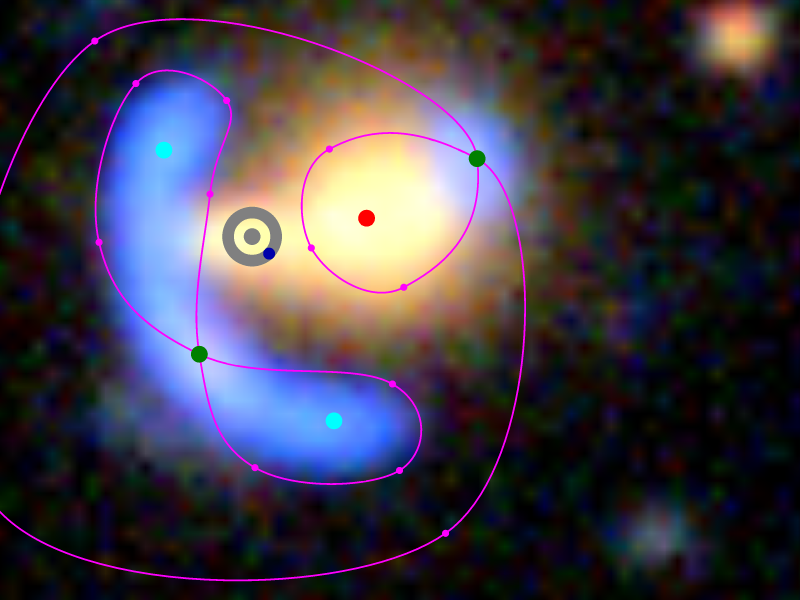
\includegraphics[width=\textwidth]{sana/#1/input}
      \caption{User input}
    \end{figure}
  \end{column}\begin{column}{0.33\textwidth}
    \begin{figure}
      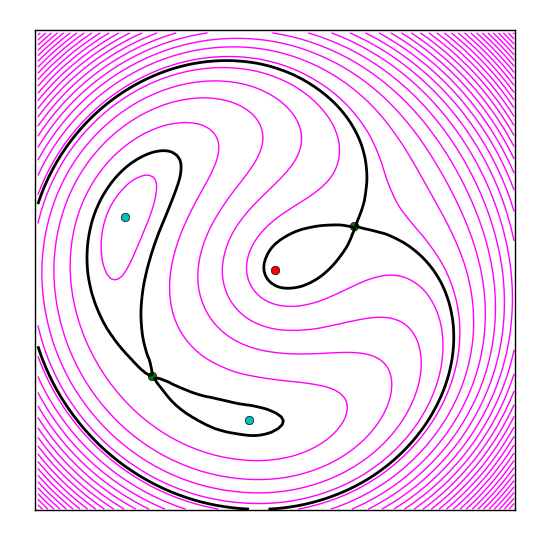
\includegraphics[width=\textwidth]{sana/#1/spaghetti2}
      \caption{Reconstructed contour lines}
    \end{figure}
  \end{column}\begin{column}{0.33\textwidth}
    \begin{figure}
      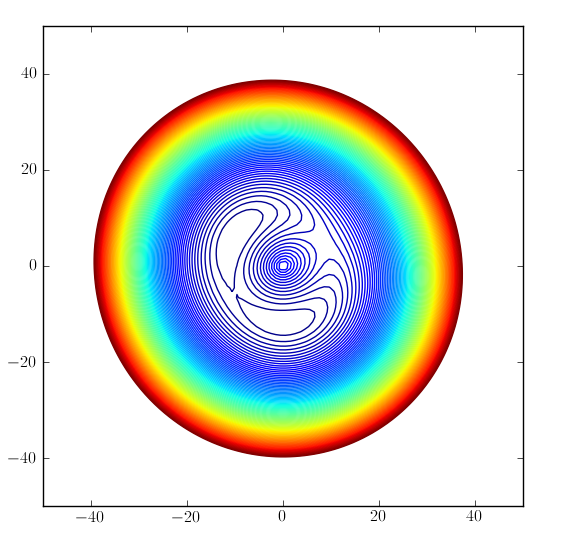
\includegraphics[width=\textwidth]{sana/#2/arriv2}
      \caption{Original contour lines}
    \end{figure}
  \end{column}\end{columns}
\end{frame}
}

\newcommand{\resframeb}[2]{
\begin{frame}
  \frametitle{Results for Model #1 (#2)}
  \begin{columns}[T]\begin{column}{0.5\textwidth}
    \begin{figure}
      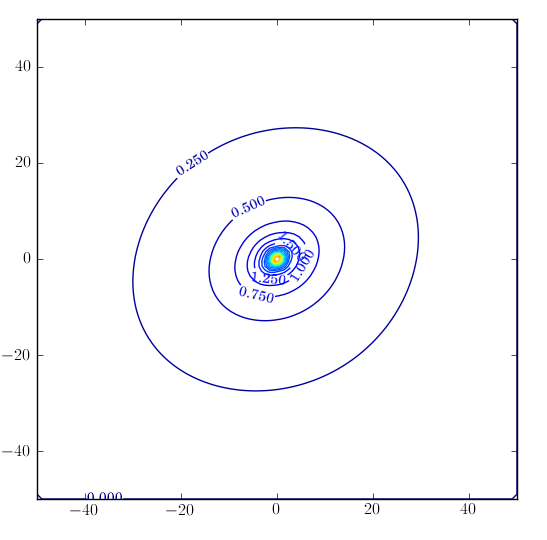
\includegraphics[height=0.8\textheight]{sana/#2/kappa2}
      \caption{Mass map $\kappa\left(x,y\right)$ of simulation}
    \end{figure}
  \end{column}\begin{column}{0.5\textwidth}
    \begin{figure}
      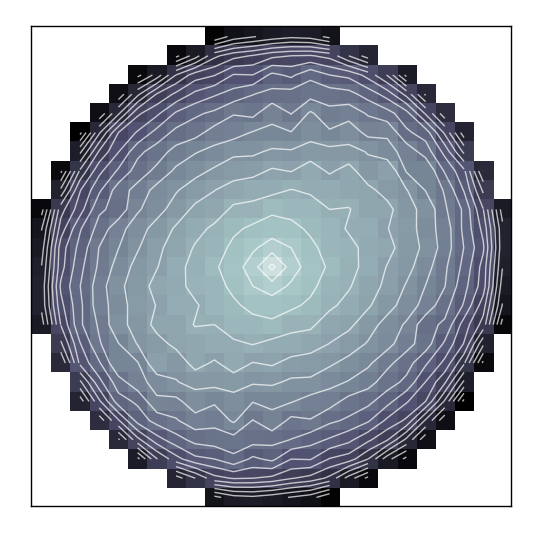
\includegraphics[width=\textwidth]{sana/#1/mass2}
      \caption{Mass map $\kappa\left(x,y\right)$ of model}
    \end{figure}
  \end{column}
  %\begin{column}{0.33\textwidth}
    %\begin{figure}
      %\includegraphics[width=\textwidth]{sana/#1/kappa_encl2}
      %\caption{Enclosed mass $\kappa\left(r\right)$}
    %\end{figure}
  %\end{column}
  \end{columns}
\end{frame}

\begin{frame}
  \frametitle{$\kappa\left(r\right)$ for Model #1 (#2)}
    \begin{figure}
      \includegraphics[height=0.8\textheight]{sana/#1/kappa_encl2}
      \caption{Enclosed mass $\kappa\left(r\right)$}
    \end{figure}
\end{frame}
}



\usepackage{appendixnumberbeamer}

\usetheme{Antibes}
%\usecolortheme{lily}
%\usefonttheme{professionalfonts}
\useinnertheme{default}
\useoutertheme{default}

\setbeamercovered{transparent}

% switch of nav
\beamertemplatenavigationsymbolsempty

%frame number
\setbeamertemplate{footline}[frame number]

\mode<presentation>

\title{SpaghettiLens}
\subtitle{Gravitational Lens Modelling}
\author[R. Küng]{Rafael Küng}
\institute[ITP -- UZH]{Institute for Theoretical Physics\\University Zurich}
\date[26.09.13]{26. Sept 2013}
%\logo{\pgfimage[width=3cm]{imgs/uzh}}
\titlegraphic{
\includegraphics[width=4cm]{imgs/uzh}}
\subject{Modelling}
\keywords{ART, Gravitational Lens, Model, Modelling}


\begin{document}
{
\setbeamertemplate{logo}{}
\begin{frame}
	\titlepage
\end{frame}
}

\section*{Motivation}
\begin{frame}
  dfg
\end{frame}



\section*{Outline}
\begin{frame}
  \frametitle{Outline}
  \tableofcontents%[pausesections]
\end{frame}


\section{Theory}

\subsection{Fermat’s Principle}

%\begin{frame}
  %\frametitle{Fermat’s Principle}
  %\begin{block}{Fermat’s Principle}
    %Time $t$ for path $X$:
    %$$t\left[X\right] = \frac{1}{c}\int_{t_1}^{t_2}n\left(\vec{x}\left(t\right)\right)\sqrt{1+\left(\frac{\text{d}\vec{x}\left(t'\right)}{\text{d}t'}\right)^2}\text{d}t'$$
    %Path $X$ where $t$ stationary.
  %\end{block}
%\end{frame}


\begin{frame}
  \frametitle{Fermat’s Principle}
  \begin{block}{Fermat’s Principle\footnote{Ghatak, Ajoy (2009), Optics}}
    %
    Rays of light traverse the path of stationary optical length\\
    with respect to variations of the path.
    
  \end{block}
\end{frame}


\ani{ani/1/n1-}{1}{45}
\ani{ani/1/n2-}{45}{50}

\subsection{ART}

\begin{frame}
  \frametitle{ART}
  \begin{block}{Einstein Field Equation\footnote{The Wall, ITP UZH}}
    %$$R_{\mu\nu} - \frac{R}{2}\, g_{\mu\nu} + \Lambda\, g_{\mu\nu} = \frac{8 \pi G}{c^4}\, T_{\mu\nu}$$
    $$G_{\mu\nu} = \Lambda\, g_{\mu\nu} + 8 \pi G\, T_{\mu\nu}$$
  \end{block}
\end{frame}


\ani{ani/2/n1-}{1}{42}
\ani{ani/2/n2-}{41}{47}
\ani{ani/2/n3-}{46}{50}


\subsection{Arrival Time Surface}

\begin{frame}
  \frametitle{Arrival Time Surface}
\end{frame}

\begin{frame}
  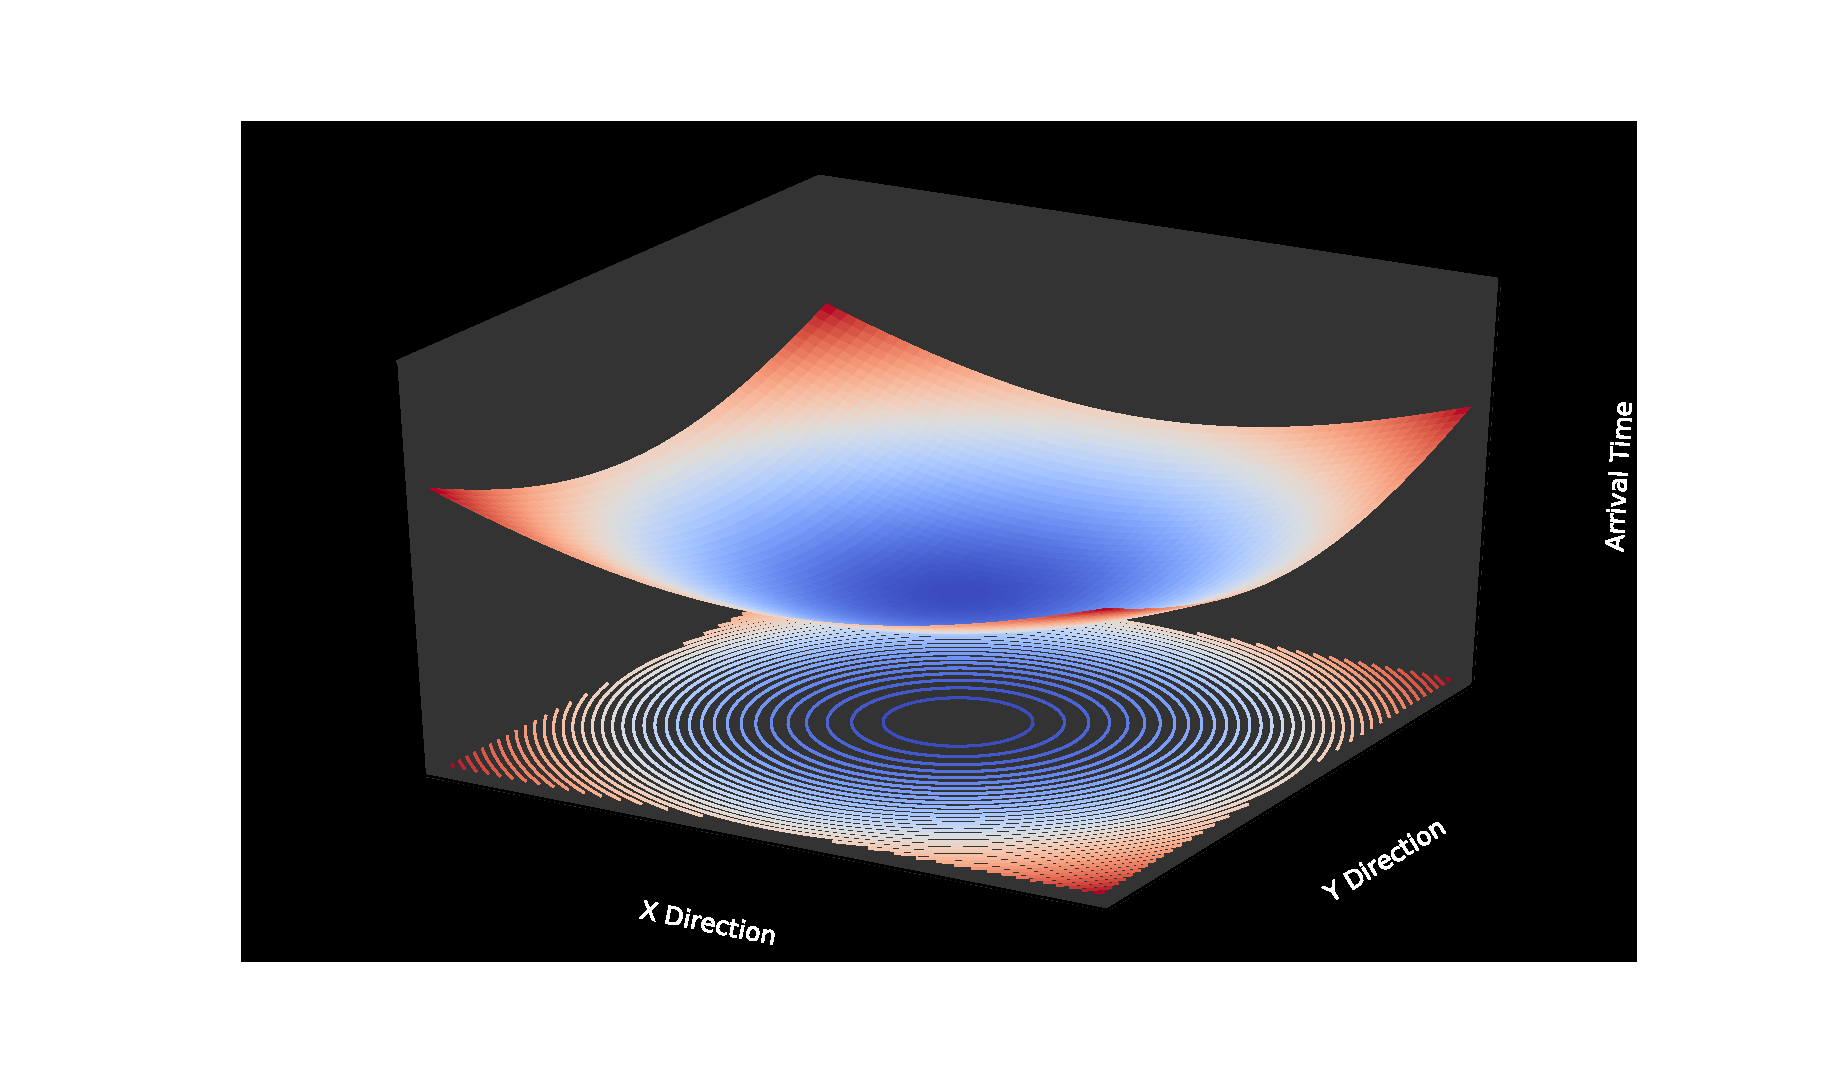
\includegraphics[height=\textheight]{imgs/fig0}
\end{frame}

\begin{frame}
  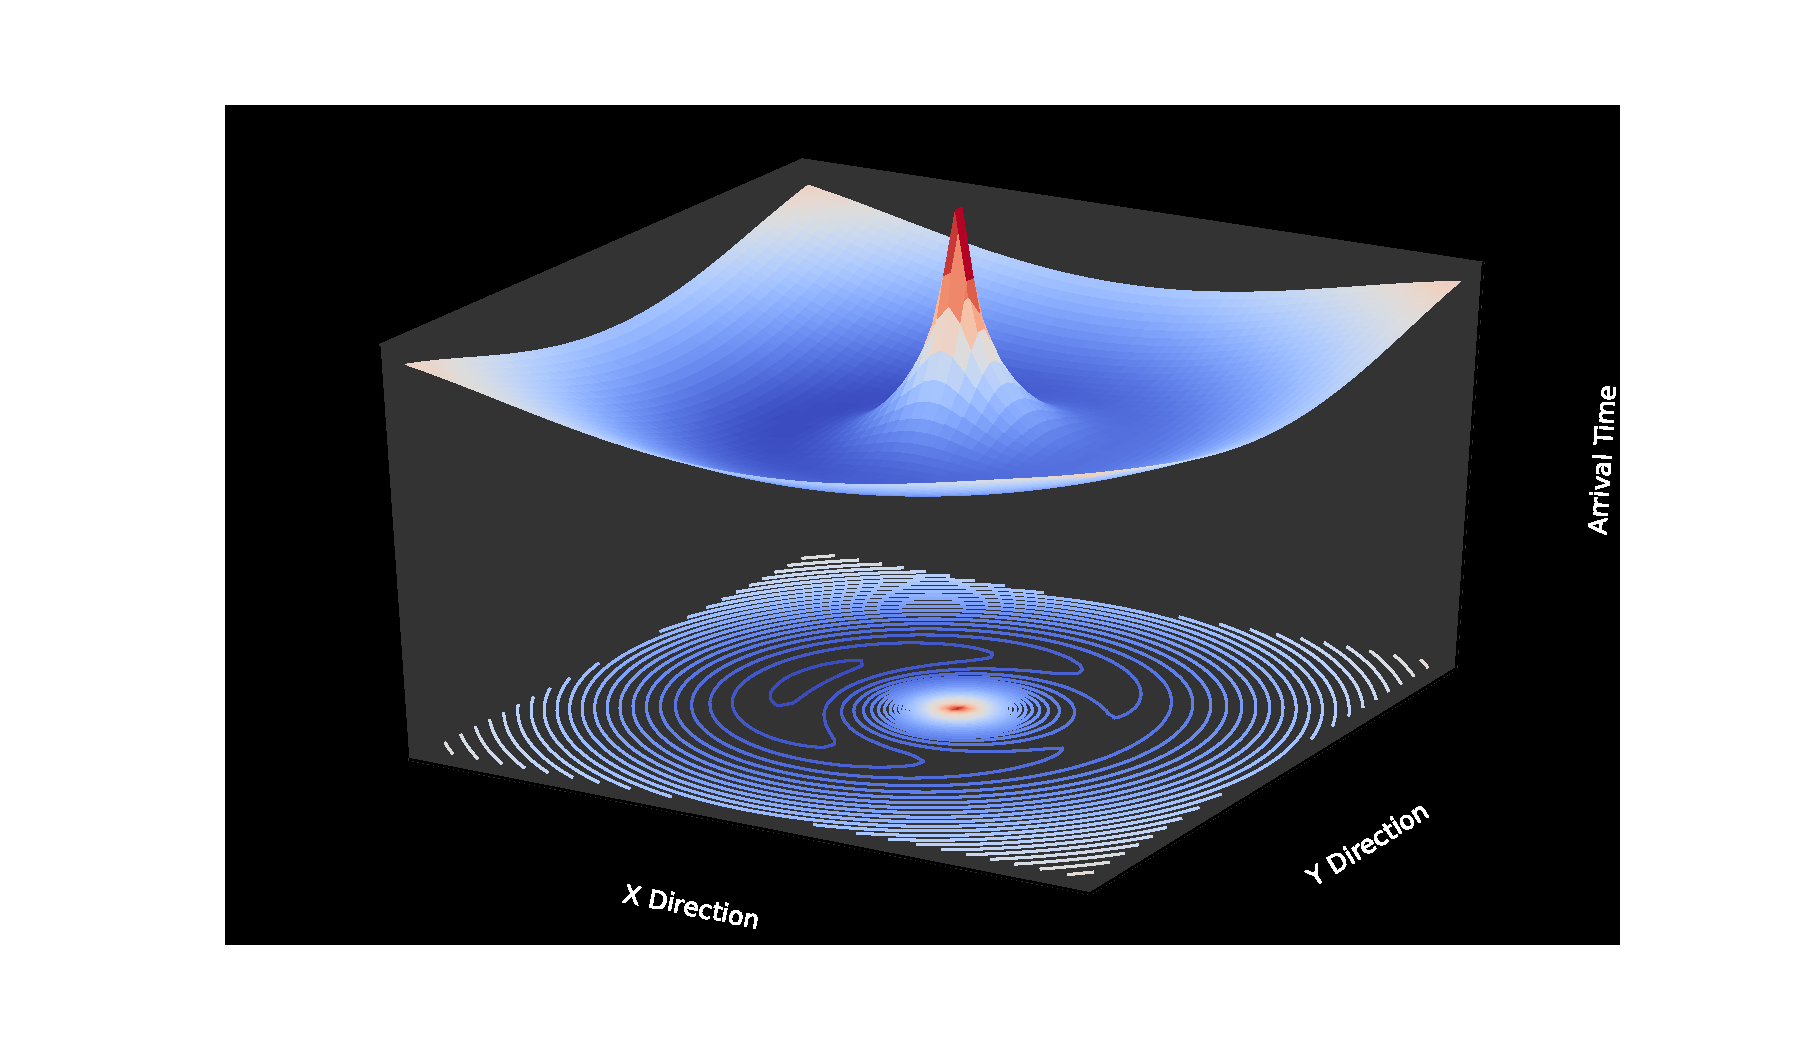
\includegraphics[height=\textheight]{imgs/fig3}
\end{frame}

%\begin{frame}
  %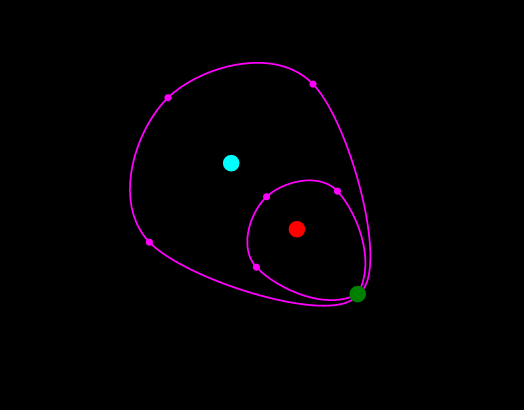
\includegraphics[width=\textwidth]{imgs/sl-3}
%\end{frame}
%
%\begin{frame}
  %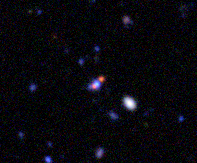
\includegraphics[width=\textwidth]{imgs/real3}
%\end{frame}

\begin{frame}
  \begin{columns}[T]
    \begin{column}{5.5cm}
      \begin{figure}
        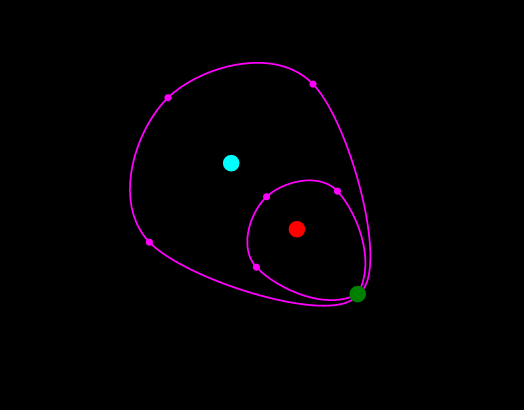
\includegraphics[width=\textwidth]{imgs/sl-3}
      \end{figure}
    \end{column}
    \begin{column}{5.5cm}
      \begin{figure}
        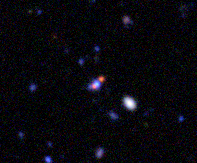
\includegraphics[width=\textwidth]{imgs/real3}
        \caption{ASW0004q9e, SpaceWarps (SW)}
      \end{figure}
    \end{column}
  \end{columns}
\end{frame}

\begin{frame}
  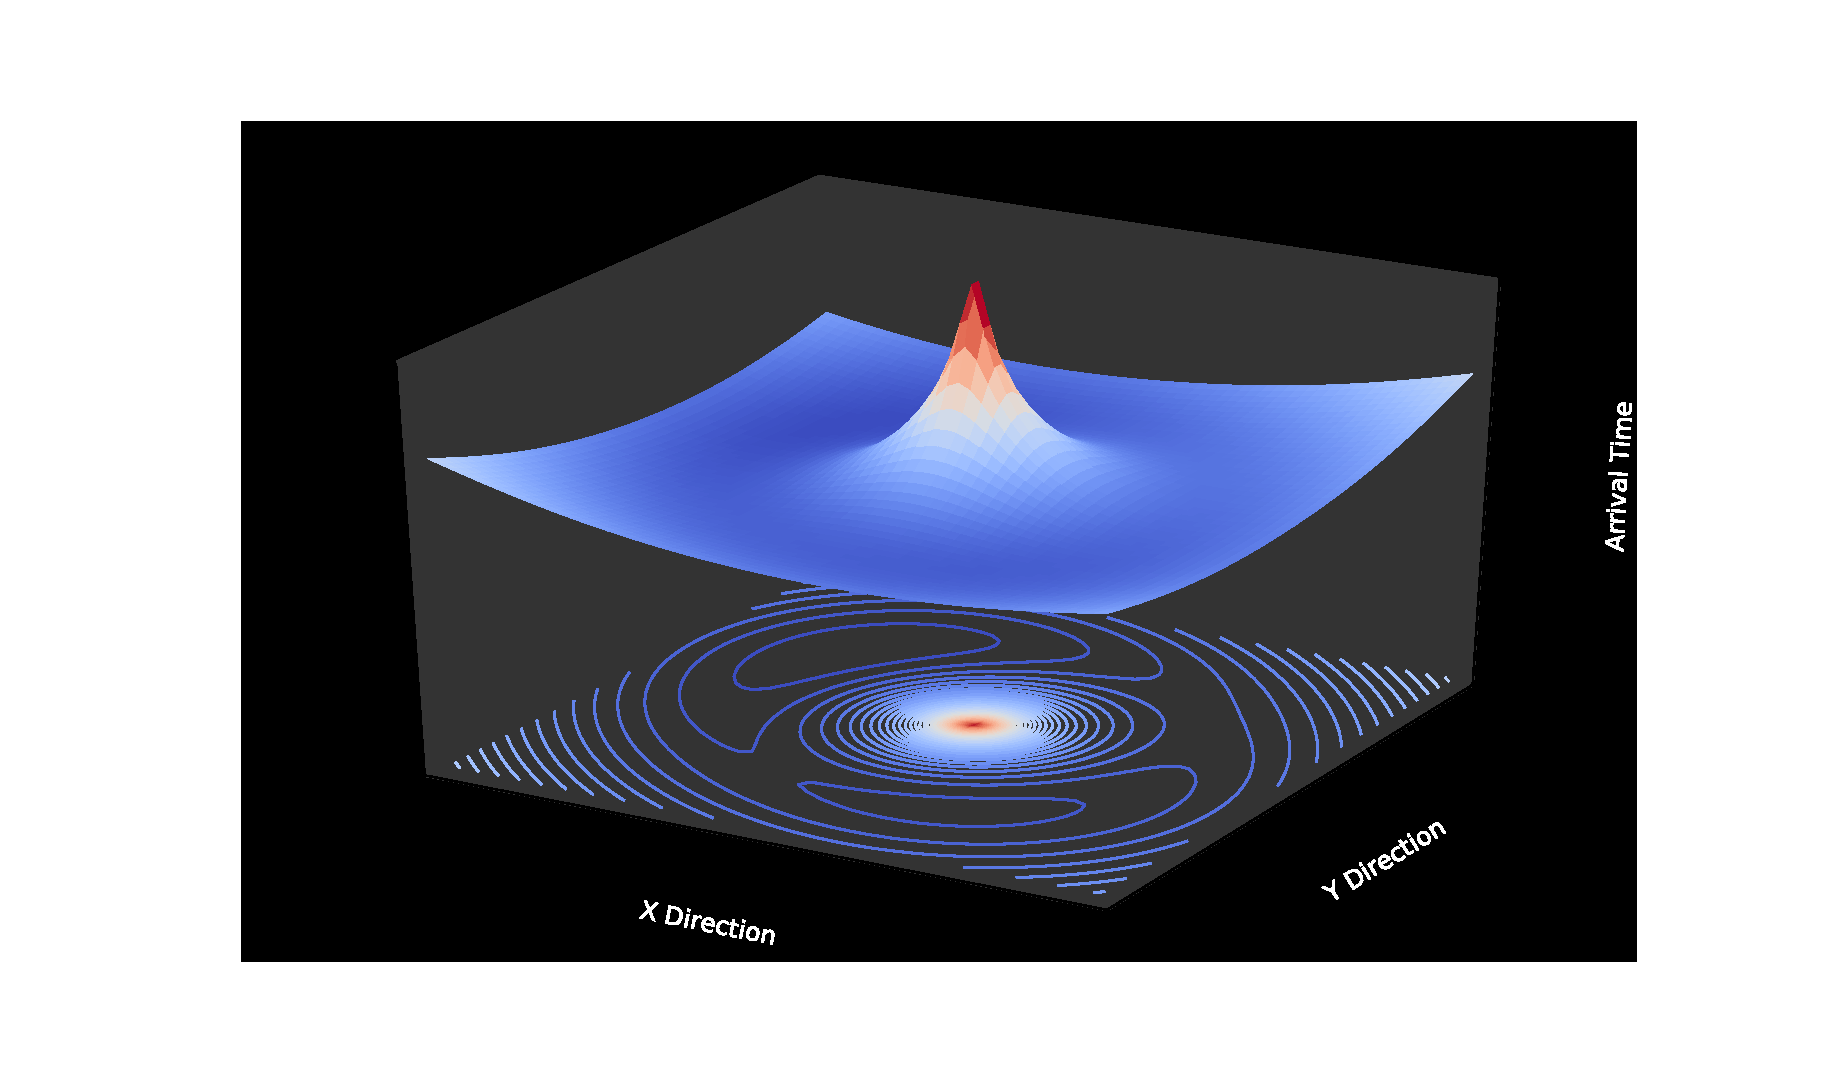
\includegraphics[width=\textwidth]{imgs/fig1}
\end{frame}

%\begin{frame}
  %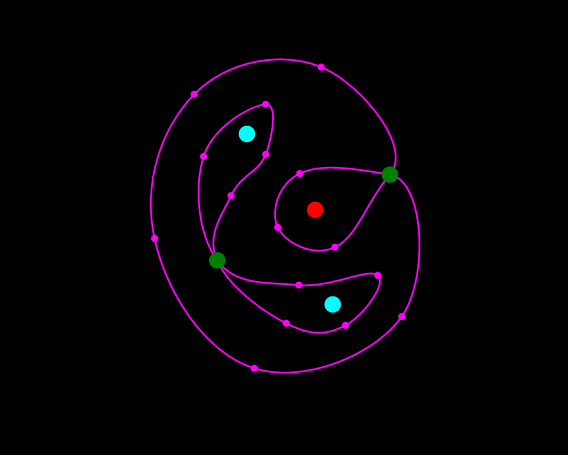
\includegraphics[width=\textwidth]{imgs/sl-1}
%\end{frame}
%
%\begin{frame}
  %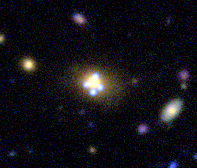
\includegraphics[width=\textwidth]{imgs/real1}
%\end{frame}

\begin{frame}
  \begin{columns}[T]
    \begin{column}{5.5cm}
      \begin{figure}
        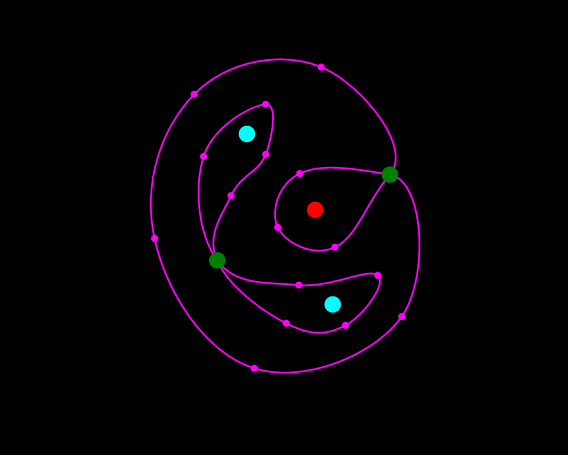
\includegraphics[width=\textwidth]{imgs/sl-1}
      \end{figure}
    \end{column}
    \begin{column}{5.5cm}
    \begin{figure}
        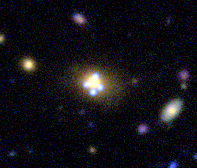
\includegraphics[width=\textwidth]{imgs/real1}
        \caption{ASW0001a8c (SW)}
      \end{figure}
    \end{column}
  \end{columns}
\end{frame}


\begin{frame}
  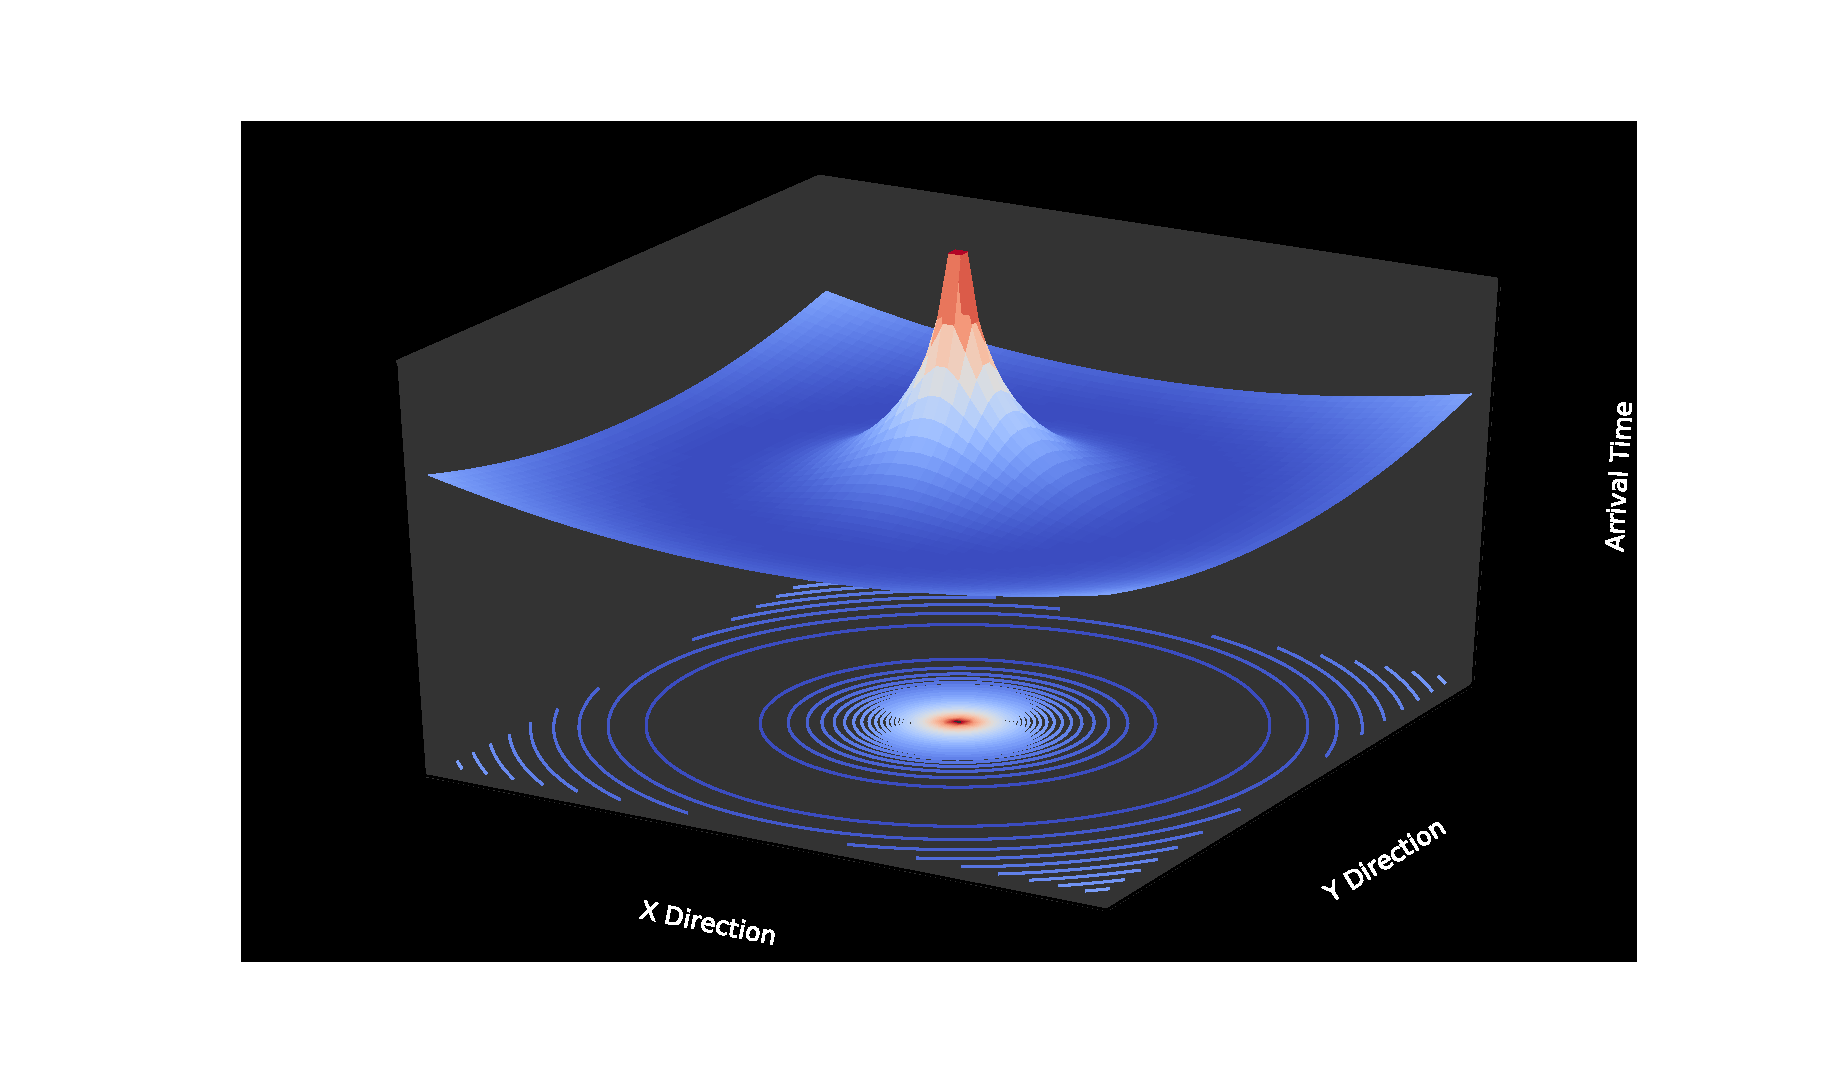
\includegraphics[width=\textwidth]{imgs/fig2}
\end{frame}

\begin{frame}
  \begin{figure}
    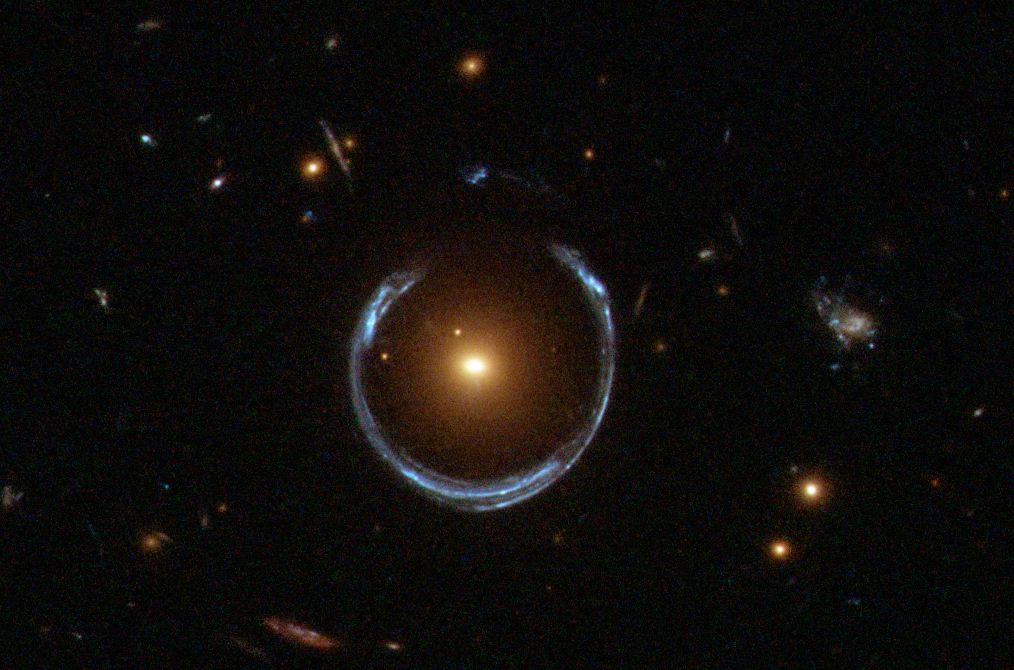
\includegraphics[height=0.9\textheight]{imgs/einsteinring}
    \caption{LRG 3-757 (2007, SDSS) Img: ESA/Hubble \& NASA}
  \end{figure}
\end{frame}

\section{SpaghettiLens}
\subsection{Demonstration}

\begin{frame}
  \frametitle{SpaghettiLens}

  \begin{columns}[c]\begin{column}{0.55\textwidth}
    \begin{itemize}
    \item Extremal Points (Images)
    \item Self Intersecting Contour Lines
    \end{itemize}
    \url{http://mite.physik.uzh.ch/}

  \end{column}\begin{column}{0.44\textwidth}
    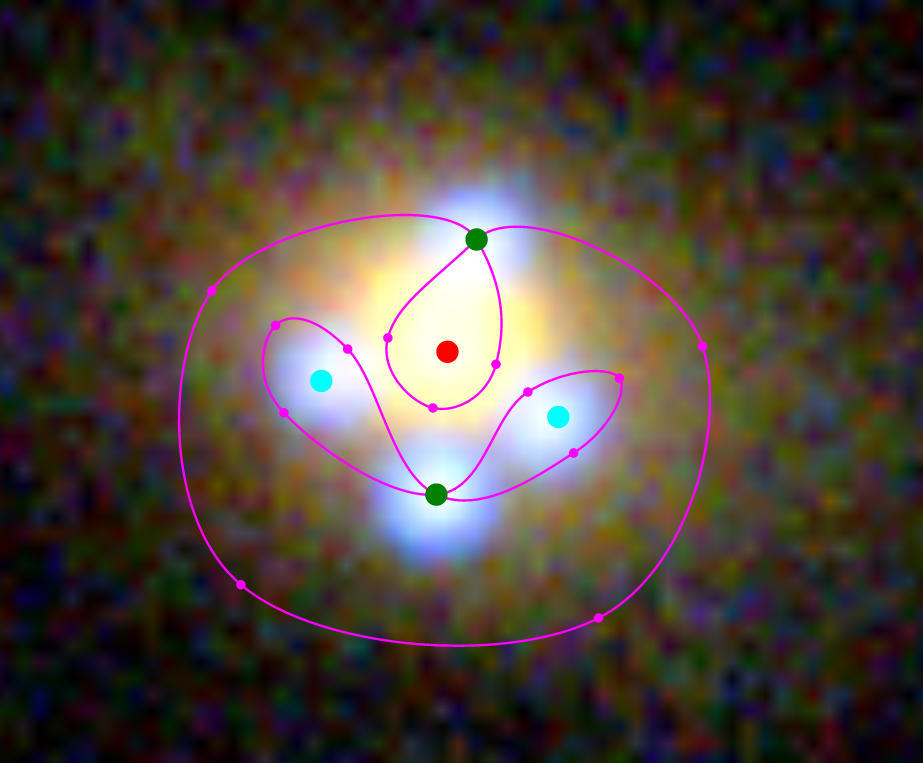
\includegraphics[width=\textwidth]{imgs/sled-1}
  \end{column}\end{columns}


\end{frame}

\subsection{Implementation}

\begin{frame}
  \frametitle{Implementation - Modules}
  \centering
  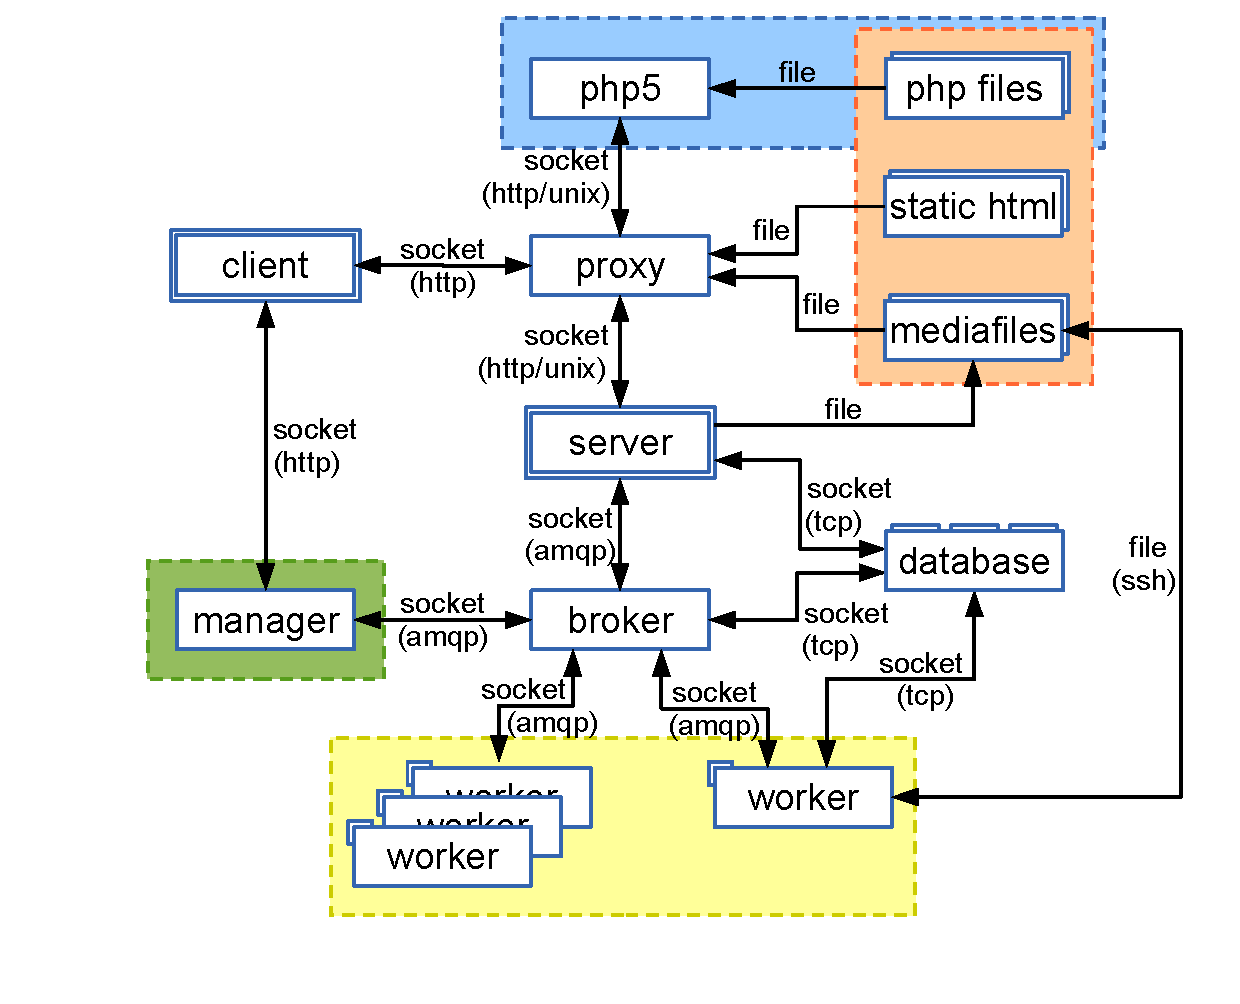
\includegraphics[height=\textheight]{imgs/whole_setup}
\end{frame}

\begin{frame}
  \frametitle{Implementation - Data Flow}
  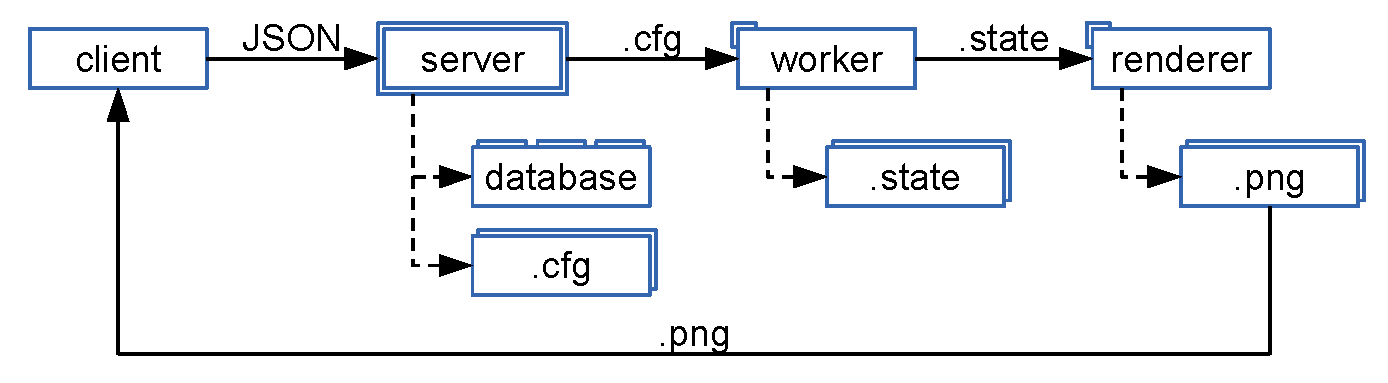
\includegraphics[width=\textwidth]{imgs/dataflow}
\end{frame}


\section{Involving Volunteers}
\subsection{Modelling Challenge}

\begin{frame}
  \frametitle{Modelling Challenge - Simulations}
  Performance evaluation of volunteers
  \begin{itemize}
    \item Selected 29 simulated lenses\footnote{Sims by Anupreeta More, using gravlens (Keeton, C. R. \& Winn, J. N. 2003, ApJ, 590, 39)}
    \item Simulation parameter hidden until evaluation
    \item Covering a range of lens configuration
  \end{itemize}
\end{frame}

\begin{frame}
  \frametitle{Modelling Challenge -- Tests}
  \begin{block}{T1: Arrival time surface}
    T1a: Correct identification of images\\
    T1b: Correct ordering
  \end{block}
  
  \begin{block}{T2: Mass Distribution}
    Comparable mass distribution $\kappa\left(x,y\right)$ of lens\\
  \end{block}
  
  \begin{itemize}
    \item Calculate enclosed mass $\kappa\left(r\right)$
    \item Determine Einstein Radius $\theta_\text{E}$ defined by $\kappa\left(\theta_\text{E}\right)=1\Rightarrow\theta_\text{E}$
    \item Compare $\theta_\text{E, sim}$ to $\theta_\text{E, model}$
  \end{itemize}

\end{frame}



\begin{frame}
  \frametitle{Results T1}
  \begin{table}\centering\begin{tabular}{llcc}\hline
 & & n & p \\
\hline
 N: & Total number of models & 119 & 1.00\\
\hline
 R1: & images approx. on right location & 110 & 0.92\\
 R2: & images with correct parity & 70 & 0.59\\
\hline
 E01: & inaccurate in arc & 21 & 0.18\\
 E02: & wrong parity in 3 img. conf. & 2 & 0.02\\
 E03: & identified 3 of 5 imgs. & 5 & 0.04\\
 E04: & modeled arc with single img. & 4 & 0.03\\
 E05: & $\pi$ rotated & 7 & 0.06\\
 E06: & $\pi$/2 rotated & 38 & 0.32\\
 E07: & missed faint img. & 1 & 0.01\\
 E08: & too many imgs in arc & 5 & 0.04\\
 E09: & missed double img & 3 & 0.03\\
 E10: & too many imgs. & 1 & 0.01\\
\hline

\end{tabular}\caption{T1 evaluation}\label{tab:stats}\end{table}
\end{frame}

\resframea{007025}{ASW0000h2m}
%\begin{frame}
  %\frametitle{Results T1 -- Details}
  %\begin{columns}[T]\begin{column}{0.33\textwidth}
    %\begin{figure}
      %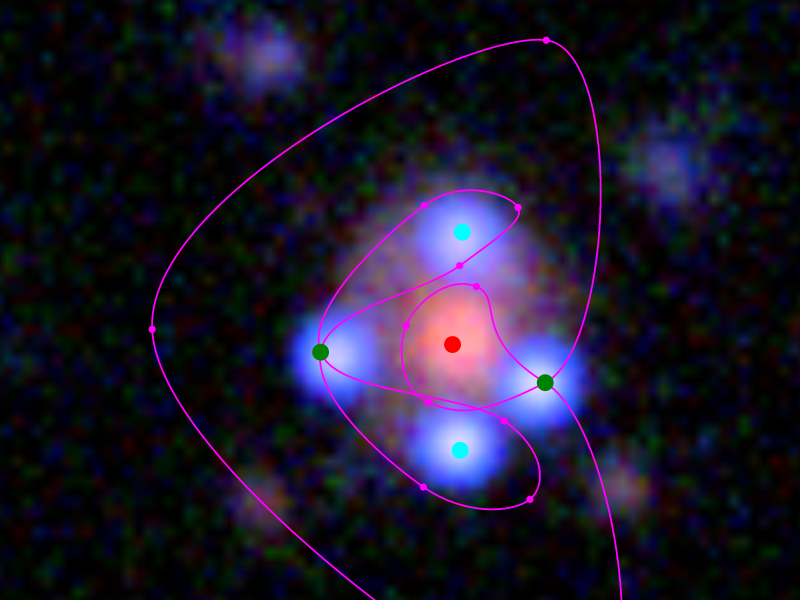
\includegraphics[width=\textwidth]{sana/007025/input}
      %\caption{User input}
    %\end{figure}
  %\end{column}\begin{column}{0.33\textwidth}
    %\begin{figure}
      %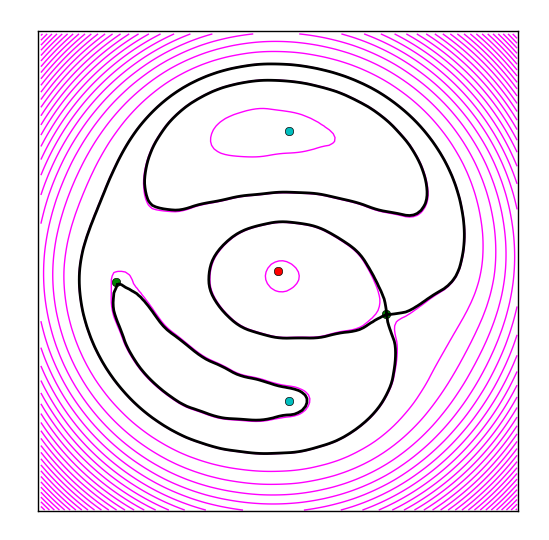
\includegraphics[width=\textwidth]{sana/007025/spaghetti2}
      %\caption{Reconstructed contour lines}
    %\end{figure}
  %\end{column}\begin{column}{0.33\textwidth}
    %\begin{figure}
      %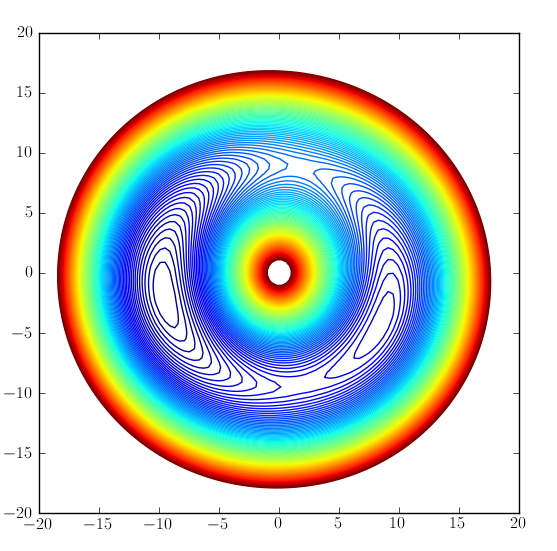
\includegraphics[width=\textwidth]{sana/ASW0000h2m/arriv2}
      %\caption{Original contour lines}
    %\end{figure}
  %\end{column}\end{columns}
%\end{frame}


\begin{frame}
  \frametitle{Results T2}
  \begin{columns}[c]\begin{column}{0.66\textwidth}
    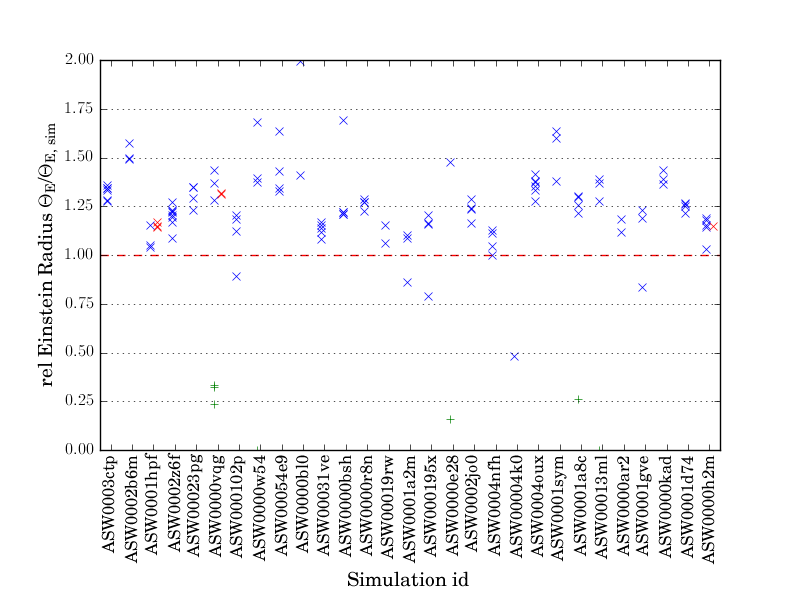
\includegraphics[height=0.9\textheight]{imgs/eR_4}
  \end{column}\begin{column}{0.33\textwidth}
    \begin{tabular}{ll}
      {\color{blue}X} & Volunteer\\
      {\color{red}X} & Professional\\
      {\color{green}+} & Rejected / Error\\
    \end{tabular}
  \end{column}\end{columns}
\end{frame}
%\begin{frame}[plain]
  %\begin{center}
    %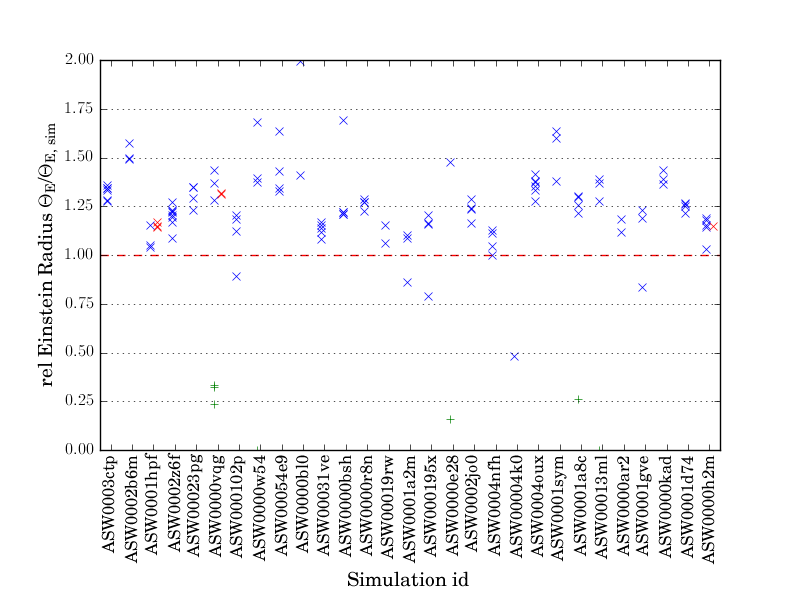
\includegraphics[height=\textheight]{imgs/eR_4}
  %\end{center}
%\end{frame}

\resframeb{007025}{ASW0000h2m}
%\begin{frame}
  %\frametitle{Results T2 -- Details}
  %\begin{columns}[T]\begin{column}{0.33\textwidth}
    %\begin{figure}
      %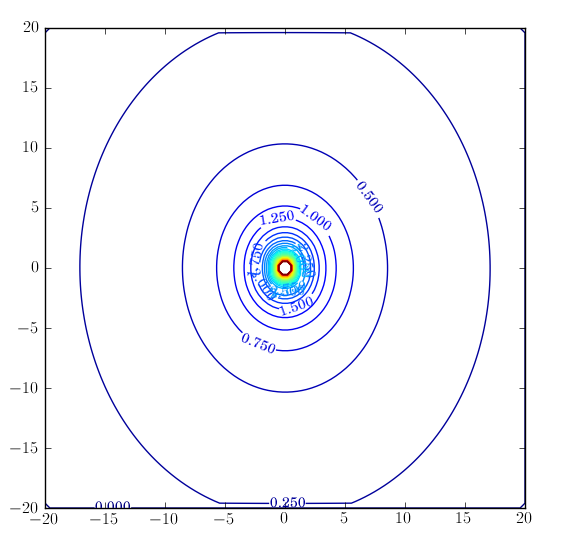
\includegraphics[width=\textwidth]{sana/ASW0000h2m/kappa2}
      %\caption{Mass map $\kappa\left(x,y\right)$ of simulation}
    %\end{figure}
  %\end{column}\begin{column}{0.33\textwidth}
    %\begin{figure}
      %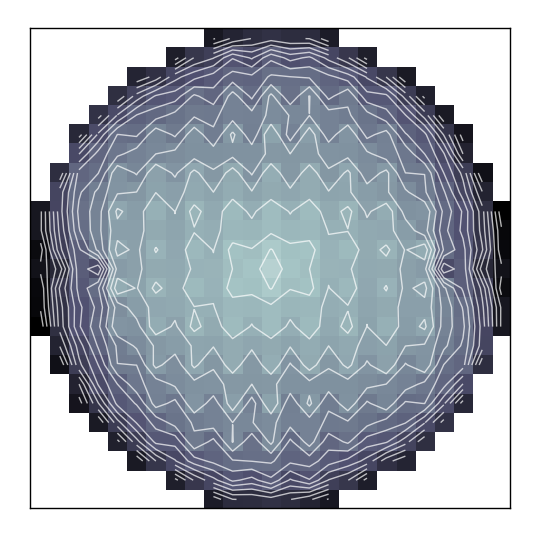
\includegraphics[width=\textwidth]{sana/007025/mass2}
      %\caption{Mass map $\kappa\left(x,y\right)$ of model}
    %\end{figure}
  %\end{column}\begin{column}{0.33\textwidth}
    %\begin{figure}
      %\includegraphics[width=\textwidth]{sana/007025/kappa_encl2}
      %\caption{Enclosed mass $\kappa\left(x,y\right)$}
    %\end{figure}
  %\end{column}\end{columns}
%\end{frame}
%
%\begin{frame}
  %\frametitle{Results T2 -- Details}
    %\begin{figure}
      %\includegraphics[height=0.8\textheight]{sana/007025/kappa_encl2}
      %\caption{Enclosed mass $\kappa\left(x,y\right)$}
    %\end{figure}
%\end{frame}


\resframea{006990}{ASW0004oux}
\resframeb{006990}{ASW0004oux}




\subsection{Collaborative Modelling}
\begin{frame}
  \frametitle{Collaborative Modelling}
\end{frame}

\section*{Conclusions}

\begin{frame}
  \frametitle{Conclusions}
  \begin{itemize}
    \item Volunteers can model lenses
    \item They do it comparably well to an scientist, if instructed
    \item They like doing it
  \end{itemize}
\end{frame}

\subsection*{Questions?}

\begin{frame}
  \frametitle{The End}
  Questions?
\end{frame}




\appendix

\begin{frame}
  \frametitle{Appendix}
\end{frame}


\end{document}